

Ce chapitre présente des fonctions essentielles en mathématiques et en sciences de l'ingénieur : les fonctions puissances, les fonctions circulaires réciproques (arcsin, arccos, arctan) et les fonctions hyperboliques (ch, sh, th) avec leurs réciproques.


\subsection*{QCM}

\begin{enumerate}
\item Pour $\alpha \in \mathbb{R}$ et $x>0$, on définit $x^\alpha$ par :
\begin{enumerate}
\item $x^\alpha = \alpha \ln(x)$
\item $x^\alpha = e^{x\ln(\alpha)}$
\item $x^\alpha = e^{\alpha \ln x}$
\item $x^\alpha = \ln(\alpha x)$
\end{enumerate}

\item La fonction $f(x)=x^{-3/2}$ est définie sur :
\begin{enumerate}
\item $\mathbb{R}$
\item $\mathbb{R}_+$
\item $\mathbb{R}_+^*$
\item $\mathbb{R}^*$
\end{enumerate}

\item La dérivée de $f(x)=x^\alpha$ pour $x>0$ est :
\begin{enumerate}
\item $x^{\alpha-1}$
\item $\alpha x^{\alpha}$
\item $\alpha x^{\alpha-1}$
\item $(\alpha-1)x^\alpha$
\end{enumerate}
\end{enumerate}


\section{Fonctions puissances}

\subsection{Définitions et propriétés}

\begin{Def}\textbf{Fonction puissance}

Une fonction puissance $f_\alpha$ est définie pour $\alpha \in \mathbb{R}$ par :
$$f_\alpha(x) = x^\alpha$$
\end{Def}

\begin{Rmq}
Selon la valeur de $\alpha$, l'ensemble de définition diffère :
\begin{itemize}
\item $x^2$, $x^3$ sont définies sur $\mathbb{R}$
\item $x^{1/2} = \sqrt{x}$ est définie sur $\mathbb{R}_+$
\item $x^{-5/2}$ est définie sur $\mathbb{R}_+^*$
\end{itemize}
\end{Rmq}

\begin{Def}\textbf{Définition générale}

Pour $\alpha \in \mathbb{R}$ et $x > 0$, on définit :
$$x^\alpha = e^{\alpha \ln x}$$
\end{Def}

\begin{Prop}\textbf{Dérivée d'une fonction puissance}

$$\forall x > 0, \forall \alpha \in \mathbb{R}, \quad (x^\alpha)' = \alpha x^{\alpha-1}$$
\end{Prop}

\paragraph{Démonstration}
À partir de $f_\alpha(x) = e^{\alpha \ln x}$ :
$$f'_\alpha(x) = (e^{\alpha \ln x})' = \left(\frac{\alpha}{x}\right) e^{\alpha \ln x} = \alpha \frac{e^{\alpha \ln x}}{e^{\ln x}} = \alpha e^{(\alpha-1)\ln x} = \alpha x^{\alpha-1}$$

\subsection{Représentations graphiques}

\begin{center}
\includegraphics[height=10cm]{images/courbe.png}
\end{center}

\vspace{1em}\hrule\vspace{1em}

\exo[1]{\textbf{QCM - Fonctions puissances}}

\begin{enumerate}
\item La dérivée de $f(x) = x^{\sqrt{2}}$ est :
\begin{multicols}{3}
\begin{enumerate}[label=\alph*.]
\item $\sqrt{2} \cdot x^{\sqrt{2}}$
\item $\sqrt{2} \cdot x^{\sqrt{2}-1}$
\item $x^{\sqrt{2}-1}$
\end{enumerate}
\end{multicols}

\item $\displaystyle\lim_{x \to 0^+} x^\pi$ vaut :
\begin{multicols}{3}
\begin{enumerate}[label=\alph*.]
\item $+\infty$
\item $0$
\item $1$
\end{enumerate}
\end{multicols}

\item $\displaystyle\lim_{x \to +\infty} x^{-1/2}$ vaut :
\begin{multicols}{3}
\begin{enumerate}[label=\alph*.]
\item $+\infty$
\item $0$
\item $-\infty$
\end{enumerate}
\end{multicols}
\end{enumerate}

\vspace{1em}\hrule\vspace{1em}

\exo[2]{\textbf{Étude de $f(x) = x^x$}}

On considère la fonction $f$ définie sur $]0,+\infty[$ par $f(x) = x^x$.

\begin{enumerate}
\item Étudier les limites de $f$ aux bornes de $]0,+\infty[$. Préciser la nature de la branche infinie.
\item Étudier le prolongement par continuité en 0, ainsi que la dérivabilité.
\item Établir les variations de $f$.
\item Tracer la courbe de $f$.
\end{enumerate}

\textit{Indication : on utilisera la définition $f(x) = e^{x \ln x}$.}

\vspace{1em}\hrule\vspace{1em}

\section{Fonctions circulaires réciproques}

\subsection{La fonction $\arcsin$}

\begin{Def}\textbf{Fonction arcsinus}

La fonction $\arcsin$ est la bijection réciproque de la fonction $\sin$ restreinte à $\left[-\frac{\pi}{2}, \frac{\pi}{2}\right]$ :
$$\arcsin : [-1, 1] \to \left[-\frac{\pi}{2}, \frac{\pi}{2}\right]$$

\textit{Notation alternative :} $\arcsin(x) = \sin^{-1}(x)$
\end{Def}

\begin{center}
\includegraphics[height=9cm]{images/courbeA.png}
\end{center}

\begin{Rmq}
$\arcsin(x)$ est l'arc dans $\left[-\frac{\pi}{2}, \frac{\pi}{2}\right]$ dont le sinus vaut $x$ :
$$\sin(\pi/6) = 1/2 \Rightarrow \arcsin(1/2) = \pi/6$$
Mais $\sin(5\pi/6) = 1/2$ et $\arcsin(1/2) \neq 5\pi/6$
\end{Rmq}

\begin{Prop}\textbf{Propriétés de $\arcsin$}

\begin{enumerate}
\item $\forall x \in \left[-\frac{\pi}{2}, \frac{\pi}{2}\right], \quad \arcsin(\sin(x)) = x$
\item $\forall x \in [-1, 1], \quad \sin(\arcsin(x)) = x$
\item $\forall x \in [-1, 1], \quad \arcsin(-x) = -\arcsin(x)$ \quad (fonction impaire)
\item \textbf{Dérivée :} $\arcsin$ est dérivable sur $]-1, 1[$ et $\arcsin'(x) = \dfrac{1}{\sqrt{1-x^2}}$
\item \textbf{Dérivée composée :} $(\arcsin(u))' = \dfrac{u'}{\sqrt{1-u^2}}$
\end{enumerate}
\end{Prop}

\vspace{1em}\hrule\vspace{1em}

\subsection{La fonction $\arccos$}

\begin{Def}\textbf{Fonction arccosinus}

La fonction $\arccos$ est la bijection réciproque de la fonction $\cos$ restreinte à $[0, \pi]$ :
$$\arccos : [-1, 1] \to [0, \pi]$$

\textit{Notation alternative :} $\arccos(x) = \cos^{-1}(x)$
\end{Def}

\begin{center}
\includegraphics[height=9cm]{images/courbeB.png}
\end{center}

\begin{Rmq}
$\arccos(x)$ est l'arc dans $[0, \pi]$ dont le cosinus vaut $x$ :
$$\cos(\pi/3) = 1/2 \Rightarrow \arccos(1/2) = \pi/3$$
Mais $\cos(-\pi/3) = 1/2$ et $\arccos(1/2) \neq -\pi/3$
\end{Rmq}

\begin{Prop}\textbf{Propriétés de $\arccos$}

\begin{enumerate}
\item $\forall x \in [0, \pi], \quad \arccos(\cos(x)) = x$
\item $\forall x \in [-1, 1], \quad \cos(\arccos(x)) = x$
\item $\forall x \in [-1, 1], \quad \arccos(-x) = \pi - \arccos(x)$
\item \textbf{Dérivée :} $\arccos$ est dérivable sur $]-1, 1[$ et $\arccos'(x) = -\dfrac{1}{\sqrt{1-x^2}}$
\item \textbf{Dérivée composée :} $(\arccos(u))' = -\dfrac{u'}{\sqrt{1-u^2}}$
\end{enumerate}
\end{Prop}

\begin{Prop}\textbf{Relations complémentaires}

\begin{itemize}
\item $\cos(\arcsin(x)) = \sqrt{1-x^2}$
\item $\sin(\arccos(x)) = \sqrt{1-x^2}$
\item \textbf{Relation fondamentale :} $\forall x \in [-1, 1], \quad \arcsin(x) + \arccos(x) = \dfrac{\pi}{2}$
\end{itemize}
\end{Prop}

\vspace{1em}\hrule\vspace{1em}

\subsection{La fonction $\arctan$}

\begin{Def}\textbf{Fonction arctangente}

La fonction $\arctan$ est la bijection réciproque de la fonction $\tan$ restreinte à $\left]-\frac{\pi}{2}, \frac{\pi}{2}\right[$ :
$$\arctan : \mathbb{R} \to \left]-\frac{\pi}{2}, \frac{\pi}{2}\right[$$

\textit{Notation alternative :} $\arctan(x) = \tan^{-1}(x)$
\end{Def}

\begin{center}
\includegraphics[height=9cm]{images/courbeC.png}
\end{center}

\begin{Rmq}
$\arctan(x)$ est l'arc dans $\left]-\frac{\pi}{2}, \frac{\pi}{2}\right[$ dont la tangente vaut $x$ :
$$\tan(\pi/4) = 1 \Rightarrow \arctan(1) = \pi/4$$
Mais $\tan(5\pi/4) = 1$ et $\arctan(1) \neq 5\pi/4$
\end{Rmq}

\begin{Prop}\textbf{Propriétés de $\arctan$}

\begin{enumerate}
\item $\forall x \in \left]-\frac{\pi}{2}, \frac{\pi}{2}\right[, \quad \arctan(\tan(x)) = x$
\item $\forall x \in \mathbb{R}, \quad \tan(\arctan(x)) = x$
\item $\forall x \in \mathbb{R}, \quad \arctan(-x) = -\arctan(x)$ \quad (fonction impaire)
\item $\forall x \in \mathbb{R}_+^*, \quad \arctan(x) + \arctan(1/x) = \dfrac{\pi}{2}$
\item $\forall x \in \mathbb{R}_-^*, \quad \arctan(x) + \arctan(1/x) = -\dfrac{\pi}{2}$
\item \textbf{Dérivée :} $\arctan$ est dérivable sur $\mathbb{R}$ et $\arctan'(x) = \dfrac{1}{1+x^2}$
\item \textbf{Dérivée composée :} $(\arctan(u))' = \dfrac{u'}{1+u^2}$
\end{enumerate}
\end{Prop}

\begin{Rmq}\textbf{Limites importantes}
$$\lim_{x \to +\infty} \arctan(x) = \frac{\pi}{2} \qquad \lim_{x \to -\infty} \arctan(x) = -\frac{\pi}{2}$$
\end{Rmq}

\vspace{1em}\hrule\vspace{1em}

\subsection{Tableau récapitulatif des fonctions circulaires réciproques}

\renewcommand{\arraystretch}{2}
\begin{center}
\begin{tabular}{|c|c|c|c|}
\hline
\textbf{Fonction} & \textbf{Domaine} & \textbf{Image} & \textbf{Dérivée} \\
\hline
$\arcsin(x)$ & $[-1, 1]$ & $\left[-\frac{\pi}{2}, \frac{\pi}{2}\right]$ & $\dfrac{1}{\sqrt{1-x^2}}$ \\
\hline
$\arccos(x)$ & $[-1, 1]$ & $[0, \pi]$ & $-\dfrac{1}{\sqrt{1-x^2}}$ \\
\hline
$\arctan(x)$ & $\mathbb{R}$ & $\left]-\frac{\pi}{2}, \frac{\pi}{2}\right[$ & $\dfrac{1}{1+x^2}$ \\
\hline
\end{tabular}
\end{center}

\vspace{1em}\hrule\vspace{1em}

\exo[1]{\textbf{QCM - Fonctions circulaires réciproques}}

\begin{enumerate}
\item $\arcsin(\sin(2\pi))$ vaut :
\begin{multicols}{3}
\begin{enumerate}[label=\alph*.]
\item $2\pi$
\item $0$
\item $\pi$
\end{enumerate}
\end{multicols}

\item $\arccos(-1/2)$ vaut :
\begin{multicols}{3}
\begin{enumerate}[label=\alph*.]
\item $-\pi/3$
\item $2\pi/3$
\item $\pi/3$
\end{enumerate}
\end{multicols}

\item La dérivée de $f(x) = \arctan(2x)$ est :
\begin{multicols}{3}
\begin{enumerate}[label=\alph*.]
\item $\dfrac{1}{1+4x^2}$
\item $\dfrac{2}{1+4x^2}$
\item $\dfrac{2}{1+2x^2}$
\end{enumerate}
\end{multicols}

\item $\arcsin(1/2) + \arccos(1/2)$ vaut :
\begin{multicols}{3}
\begin{enumerate}[label=\alph*.]
\item $\pi/3$
\item $\pi/2$
\item $\pi$
\end{enumerate}
\end{multicols}
\end{enumerate}

\vspace{1em}\hrule\vspace{1em}

\exo[2]{\textbf{Calculs de dérivées}}

Calculer la dérivée des fonctions suivantes :

\begin{multicols}{2}
\begin{enumerate}
\item $f(x) = \arcsin(2x-1)$
\item $g(x) = \arccos(x^2)$
\item $h(x) = \arctan(\sqrt{x})$
\item $k(x) = x \arcsin(x) + \sqrt{1-x^2}$
\end{enumerate}
\end{multicols}

\vspace{1em}\hrule\vspace{1em}

\exo[2]{\textbf{Concavité}}

Étudier la fonction $g(x) = \arctan(\sqrt{x})$. Préciser la concavité.

\vspace{1em}\hrule\vspace{1em}

\exo[2]{\textbf{Égalité célèbre}}

Pour $x \neq 0$, on pose $f(x) = \arctan(x) + \arctan\left(\dfrac{1}{x}\right)$.

\begin{enumerate}
\item Calculer $f'(x)$ pour $x \neq 0$.
\item En déduire que :
$$\forall x \in \mathbb{R}_+^*, \quad \arctan(x) + \arctan\left(\frac{1}{x}\right) = \frac{\pi}{2}$$
$$\forall x \in \mathbb{R}_-^*, \quad \arctan(x) + \arctan\left(\frac{1}{x}\right) = -\frac{\pi}{2}$$
\end{enumerate}

\vspace{1em}\hrule\vspace{1em}

\exo[2]{\textbf{Intervalle}}

On pose $\alpha = \arctan(4/3)$ et $\beta = 2\arctan(1/2)$.

\begin{enumerate}
\item Démontrer que $\alpha \in \left]-\frac{\pi}{2}, \frac{\pi}{2}\right[$ et $\beta \in \left]-\frac{\pi}{2}, \frac{\pi}{2}\right[$.

\textit{Indication : pour $\beta$, penser à encadrer 1/2 entre deux valeurs adéquates.}

\item Comparer $\tan(\alpha)$ et $\tan(\beta)$.

\textit{On rappelle que $\tan(2a) = \dfrac{2\tan a}{1-\tan^2 a}$.}

\item Conclure.
\end{enumerate}

\vspace{1em}\hrule\vspace{1em}

\exo[2]{\textbf{Point d'inflexion}}

On considère la fonction $f : x \mapsto \arctan(2-x)$.

\begin{enumerate}
\item Déterminer l'ensemble de définition $D_f$ de $f$ et les limites de $f$ aux bornes de $D_f$.
\item Étudier les variations de $f$.
\item Étudier la concavité de $f$. Préciser la tangente au point d'inflexion.
\item Représenter la courbe de $f$.
\end{enumerate}

\vspace{1em}\hrule\vspace{1em}

\exo[3]{\textbf{Dérivabilité}}

On considère la fonction $f : x \mapsto \arctan\sqrt{|x|}$.

\begin{enumerate}
\item Déterminer l'ensemble de définition $D_f$ de $f$.
\item Montrer que $f$ est paire.
\item Déterminer les limites aux bornes de $D_f$.
\item Étudier la dérivabilité de $f$ à droite en 0.
\item Étudier les variations de $f$ sur $\mathbb{R}_+$.
\item Représenter la courbe de $f$.
\end{enumerate}

\vspace{1em}\hrule\vspace{1em}

\exo[3]{\textbf{Tangentes}}

On considère la fonction $f : x \mapsto \dfrac{x}{1+x^2} - \arctan x$.

\begin{enumerate}
\item Déterminer l'ensemble de définition $D_f$ de $f$ et les limites de $f$ aux bornes de $D_f$.
\item Étudier les variations et la concavité de $f$. Préciser les tangentes aux points d'inflexion.
\item Représenter la courbe de $f$.
\end{enumerate}

\vspace{1em}\hrule\vspace{1em}

\subsection*{QCM}

\begin{enumerate}
\item L'image de la fonction $\arcsin$ est :
\begin{enumerate}
\item $[-1,1]$
\item $[0,\pi]$
\item $\left[-\dfrac{\pi}{2},\dfrac{\pi}{2}\right]$
\item $\mathbb{R}$
\end{enumerate}

\item Pour tout $x \in [-1,1]$, on a :
\begin{enumerate}
\item $\arccos(\cos(x))=x$
\item $\sin(\arcsin(x))=x$
\item $\arcsin(x)+\arccos(x)=\pi$
\item $\arctan(\tan(x))=x$
\end{enumerate}

\item La dérivée de $\arctan(x)$ est :
\begin{enumerate}
\item $\dfrac{1}{\sqrt{1-x^2}}$
\item $\dfrac{1}{1-x^2}$
\item $\dfrac{1}{1+x^2}$
\item $\sqrt{1+x^2}$
\end{enumerate}

\item La limite de $\arctan(x)$ lorsque $x\to+\infty$ vaut :
\begin{enumerate}
\item $+\infty$
\item $1$
\item $\pi$
\item $\dfrac{\pi}{2}$
\end{enumerate}
\end{enumerate}


\section{Fonctions hyperboliques}

\subsection{Définitions}

\begin{Def}\textbf{Fonctions hyperboliques}

On définit sur $\mathbb{R}$ les fonctions cosinus hyperbolique, sinus hyperbolique et tangente hyperbolique :
$$\text{ch}(x) = \cosh(x) = \frac{e^x + e^{-x}}{2}$$
$$\text{sh}(x) = \sinh(x) = \frac{e^x - e^{-x}}{2}$$
$$\text{th}(x) = \tanh(x) = \frac{\text{sh}(x)}{\text{ch}(x)} = \frac{e^x - e^{-x}}{e^x + e^{-x}}$$
\end{Def}

\begin{Rmq}
Les fonctions $\text{ch}(x)$ et $\text{sh}(x)$ sont les solutions paramétriques de l'hyperbole équilatère :
$$X^2 - Y^2 = 1$$

\begin{center}
\includegraphics[scale=0.7]{images/courbeHyperbole}
\end{center}
\end{Rmq}

\begin{Rmq}
On peut aussi écrire : $\text{th}(x) = \dfrac{e^{2x}-1}{e^{2x}+1}$
\end{Rmq}

\subsection{Parité et relations remarquables}

\begin{Prop}\textbf{Parité}

\begin{itemize}
\item $\text{ch}(-x) = \text{ch}(x)$ : la fonction ch est \textbf{paire}
\item $\text{sh}(-x) = -\text{sh}(x)$ : la fonction sh est \textbf{impaire}
\item $\text{th}(-x) = -\text{th}(x)$ : la fonction th est \textbf{impaire}
\end{itemize}
\end{Prop}

\begin{Prop}\textbf{Relations remarquables}

\begin{enumerate}
\item $\text{ch}(x) + \text{sh}(x) = e^x$
\item $\text{ch}(x) - \text{sh}(x) = e^{-x}$
\end{enumerate}
\end{Prop}

\subsection{Trigonométrie hyperbolique}

\begin{Prop}\textbf{Relations fondamentales}

\begin{enumerate}
\item $\text{ch}^2(x) - \text{sh}^2(x) = 1$ \quad (analogue de $\cos^2 + \sin^2 = 1$)
\item $\text{ch}^2(x) + \text{sh}^2(x) = \text{ch}(2x)$
\item $2\,\text{ch}(x)\,\text{sh}(x) = \text{sh}(2x)$
\end{enumerate}
\end{Prop}

\paragraph{Démonstration de la première relation}
$$\text{ch}^2(x) - \text{sh}^2(x) = \left(\frac{e^x + e^{-x}}{2}\right)^2 - \left(\frac{e^x - e^{-x}}{2}\right)^2 = \frac{(e^x + e^{-x})^2 - (e^x - e^{-x})^2}{4}$$
$$= \frac{e^{2x} + 2 + e^{-2x} - e^{2x} + 2 - e^{-2x}}{4} = \frac{4}{4} = 1$$

\subsection{Dérivées}

\begin{Prop}\textbf{Dérivées des fonctions hyperboliques}

$$\text{ch}'(x) = \text{sh}(x)$$
$$\text{sh}'(x) = \text{ch}(x)$$
$$\text{th}'(x) = \frac{1}{\text{ch}^2(x)} = 1 - \text{th}^2(x)$$
\end{Prop}

\begin{Rmq}
Contrairement aux fonctions trigonométriques usuelles, on a $\text{sh}'(x) = \text{ch}(x)$ (sans signe moins).
\end{Rmq}

\subsection{Limites et équivalents}

\begin{Prop}\textbf{Limites en $\pm\infty$}

$$\lim_{x \to +\infty} \text{ch}(x) = +\infty \qquad \lim_{x \to -\infty} \text{ch}(x) = +\infty$$
$$\lim_{x \to +\infty} \text{sh}(x) = +\infty \qquad \lim_{x \to -\infty} \text{sh}(x) = -\infty$$
$$\lim_{x \to +\infty} \text{th}(x) = 1 \qquad \lim_{x \to -\infty} \text{th}(x) = -1$$

La fonction th admet deux asymptotes horizontales : $y = 1$ et $y = -1$.
\end{Prop}

\begin{Prop}\textbf{Équivalents}

\begin{itemize}
\item $\text{ch}(x) \underset{+\infty}{\sim} \dfrac{e^x}{2}$ et $\text{ch}(x) \underset{-\infty}{\sim} \dfrac{e^{-x}}{2}$ et $\text{ch}(x) - 1 \underset{0}{\sim} \dfrac{x^2}{2}$
\item $\text{sh}(x) \underset{+\infty}{\sim} \dfrac{e^x}{2}$ et $\text{sh}(x) \underset{-\infty}{\sim} -\dfrac{e^{-x}}{2}$ et $\text{sh}(x) \underset{0}{\sim} x$
\item $\text{th}(x) \underset{+\infty}{\sim} 1$ et $\text{th}(x) \underset{0}{\sim} x$
\end{itemize}
\end{Prop}

\subsection{Variations}

\begin{minipage}[t]{0.45\linewidth}
\begin{center}
\textbf{Fonction ch}
\end{center}
\begin{tikzpicture}
\tkzTabInit{$x$ /1, $\mathrm{ch}'(x)$ /1.5, $\mathrm{ch}$ /2.5}{$-\infty$, $0$, $+\infty$}
\tkzTabLine{, -, z, +, }
\tkzTabVar{+/ $+\infty$, -/ $1$, +/ $+\infty$}
\end{tikzpicture}
\end{minipage}
\hfill
\begin{minipage}[t]{0.45\linewidth}
\begin{center}
\textbf{Fonction sh}
\end{center}
\begin{tikzpicture}
\tkzTabInit[lgt=2, espcl=2.5]{$x$ /1, $\mathrm{sh}'(x)$ /1.5, $\mathrm{sh}$ /2.5}{$-\infty$, $0$, $+\infty$}
\tkzTabLine{, , +, }
\tkzTabVar{-/ $-\infty$, R/ , +/ $+\infty$}
\tkzTabIma{1}{3}{2}{0}
\end{tikzpicture}
\end{minipage}

\vspace{1em}

\begin{center}
\textbf{Fonction th}
\end{center}
\begin{tikzpicture}
\tkzTabInit[lgt=2, espcl=3]{$x$ /1, $\mathrm{th}'(x)$ /1.5, $\mathrm{th}$ /2.5}{$-\infty$, $0$, $+\infty$}
\tkzTabLine{, , +, }
\tkzTabVar{-/ $-1$, R/ , +/ $1$}
\tkzTabIma{1}{3}{2}{0}
\end{tikzpicture}

\subsection{Courbes}

\begin{Rmq}\textbf{Comportement de ch et sh}
\begin{enumerate}
\item $\text{ch}(x) - \text{sh}(x) = e^{-x} > 0$, donc $\text{ch}(x) > \text{sh}(x)$ pour tout $x$
\item $\displaystyle\lim_{x \to +\infty} (\text{ch}(x) - \text{sh}(x)) = \lim_{x \to +\infty} e^{-x} = 0$

Les courbes de ch et sh sont asymptotes l'une de l'autre en $+\infty$.
\end{enumerate}
\end{Rmq}

\begin{center}
\includegraphics[height=10cm]{images/courbeD.png}
\end{center}

\vspace{1em}\hrule\vspace{1em}

\subsection{Tableau récapitulatif}

\renewcommand{\arraystretch}{2}
\begin{center}
\begin{tabular}{|c|c|c|c|c|}
\hline
\textbf{Fonction} & \textbf{Domaine} & \textbf{Parité} & \textbf{Dérivée} & \textbf{Limites} \\
\hline
$\text{ch}(x)$ & $\mathbb{R}$ & paire & $\text{sh}(x)$ & $+\infty$ \\
\hline
$\text{sh}(x)$ & $\mathbb{R}$ & impaire & $\text{ch}(x)$ & $\pm\infty$ \\
\hline
$\text{th}(x)$ & $\mathbb{R}$ & impaire & $\dfrac{1}{\text{ch}^2(x)}$ & $\pm 1$ \\
\hline
\end{tabular}
\end{center}

\vspace{1em}\hrule\vspace{1em}

\exo[1]{\textbf{QCM - Fonctions hyperboliques}}

\begin{enumerate}
\item $\text{ch}(0)$ vaut :
\begin{multicols}{3}
\begin{enumerate}[label=\alph*.]
\item $0$
\item $1$
\item $e$
\end{enumerate}
\end{multicols}

\item La dérivée de $\text{sh}(2x)$ est :
\begin{multicols}{3}
\begin{enumerate}[label=\alph*.]
\item $\text{ch}(2x)$
\item $2\,\text{ch}(2x)$
\item $-2\,\text{ch}(2x)$
\end{enumerate}
\end{multicols}

\item $\text{ch}^2(x) - \text{sh}^2(x)$ vaut :
\begin{multicols}{3}
\begin{enumerate}[label=\alph*.]
\item $0$
\item $1$
\item $2$
\end{enumerate}
\end{multicols}

\item $\displaystyle\lim_{x \to +\infty} \text{th}(x)$ vaut :
\begin{multicols}{3}
\begin{enumerate}[label=\alph*.]
\item $0$
\item $1$
\item $+\infty$
\end{enumerate}
\end{multicols}
\end{enumerate}

\vspace{1em}\hrule\vspace{1em}

\exo[2]{\textbf{Constante}}

Démontrer que la fonction $f : x \mapsto \arcsin(\text{th}(x)) - 2\arctan(e^x)$ est constante.

\textit{Calculer $f'(x)$ puis déterminer la constante en calculant $f(0)$.}

\vspace{1em}\hrule\vspace{1em}

\exo[2]{\textbf{Simplification}}

On considère la fonction $f$ définie par : $f(x) = \ln\sqrt{\dfrac{1+\text{th}(x)}{1-\text{th}(x)}}$.

\begin{enumerate}
\item Déterminer $D_f$.
\item Donner une expression simplifiée de $f(x)$.
\end{enumerate}

\vspace{1em}\hrule\vspace{1em}

\exo[2]{\textbf{Parité et variations}}

On considère la fonction $f$ définie par : $f(x) = \text{th}(x) - \dfrac{1}{3}\text{th}^3(x)$.

\begin{enumerate}
\item Déterminer $D_f$.
\item Étudier la parité de $f$.
\item Donner les limites de $f(x)$ aux bornes de $D_f$.
\item Étudier $f$.
\item Tracer la courbe de $f$.
\end{enumerate}

\vspace{1em}\hrule\vspace{1em}

\exo[2]{\textbf{Asymptotes obliques}}

On considère la fonction $f : x \mapsto x - \text{th}(x)$.

\begin{enumerate}
\item Déterminer $D_f$.
\item Étudier la parité de $f$.
\item Donner les limites de $f(x)$ aux bornes de $D_f$. Préciser les asymptotes.
\item Étudier $f$.
\item Tracer la courbe de $f$.
\end{enumerate}

\vspace{1em}\hrule\vspace{1em}

\subsection*{QCM}

\begin{enumerate}
\item La fonction $\text{ch}$ est :
\begin{enumerate}
\item impaire
\item périodique
\item paire
\item bornée
\end{enumerate}

\item La relation fondamentale de la trigonométrie hyperbolique est :
\begin{enumerate}
\item $\text{ch}^2(x)+\text{sh}^2(x)=1$
\item $\text{ch}^2(x)-\text{sh}^2(x)=1$
\item $\text{sh}^2(x)-\text{ch}^2(x)=1$
\item $\text{th}^2(x)=1$
\end{enumerate}

\item La dérivée de $\text{th}(x)$ est :
\begin{enumerate}
\item $\text{ch}(x)$
\item $1-\text{th}^2(x)$
\item $\dfrac{1}{1+x^2}$
\item $\text{sh}(x)$
\end{enumerate}

\item La fonction $\text{th}$ admet :
\begin{enumerate}
\item une asymptote verticale
\item deux asymptotes horizontales
\item une asymptote oblique
\item aucune asymptote
\end{enumerate}
\end{enumerate}


\section{Fonctions hyperboliques réciproques}

\subsection{Fonction Argsh (argument sinus hyperbolique)}

\begin{Def}\textbf{Fonction Argsh}

La fonction $\text{Argsh}$ est la bijection réciproque de la fonction sh :
$$\text{Argsh} : \mathbb{R} \to \mathbb{R}$$
\end{Def}

\begin{Rmq}
$\forall x \in \mathbb{R}, \quad \text{sh}(\text{Argsh}(x)) = x$ et $\text{Argsh}(\text{sh}(x)) = x$
\end{Rmq}

\begin{minipage}[t]{0.45\linewidth}
\begin{tikzpicture}
\tkzTabInit[lgt=2.5, espcl=2.5]{$x$ /1, $\mathrm{Argsh}'(x)$ /1.5, $\mathrm{Argsh}$ /2.5}{$-\infty$, $0$, $+\infty$}
\tkzTabLine{, , +, }
\tkzTabVar{-/ $-\infty$, R/ , +/ $+\infty$}
\tkzTabIma{1}{3}{2}{0}
\end{tikzpicture}
\end{minipage}
\hfill
\begin{minipage}[t]{0.45\linewidth}
\begin{center}
\includegraphics[height=5cm]{images/courbeE.png}
\end{center}
\end{minipage}

\subsection{Fonction Argch (argument cosinus hyperbolique)}

\begin{Def}\textbf{Fonction Argch}

La fonction $\text{Argch}$ est la bijection réciproque de la fonction ch restreinte à $[0, +\infty[$ :
$$\text{Argch} : [1, +\infty[ \to [0, +\infty[$$
\end{Def}

\begin{Rmq}
$\forall x \geq 1, \quad \text{ch}(\text{Argch}(x)) = x$ et $\forall x \geq 0, \quad \text{Argch}(\text{ch}(x)) = x$

\textcolor{red}{\textbf{Attention :}} $\text{Argch}(\text{ch}(x))$ est définie pour tout $x \in \mathbb{R}$ mais ne vaut exactement $x$ que lorsque $x \geq 0$.
\end{Rmq}

\begin{minipage}[t]{0.45\linewidth}
\begin{tikzpicture}
\tkzTabInit[lgt=2.5, espcl=2.5]{$x$ /1, $\mathrm{Argch}'(x)$ /1.5, $\mathrm{Argch}$ /2.5}{$1$, , $+\infty$}
\tkzTabLine{d, , +, }
\tkzTabVar{-/ $0$, R/ , +/ $+\infty$}
\end{tikzpicture}
\end{minipage}
\hfill
\begin{minipage}[t]{0.45\linewidth}
\begin{center}
\includegraphics[height=5cm]{images/courbeF.png}
\end{center}
\end{minipage}

\subsection{Fonction Argth (argument tangente hyperbolique)}

\begin{Def}\textbf{Fonction Argth}

La fonction $\text{Argth}$ est la bijection réciproque de la fonction th :
$$\text{Argth} : ]-1, 1[ \to \mathbb{R}$$
\end{Def}

\begin{Rmq}
$\forall x \in ]-1, 1[, \quad \text{th}(\text{Argth}(x)) = x$ et $\forall x \in \mathbb{R}, \quad \text{Argth}(\text{th}(x)) = x$
\end{Rmq}

\begin{minipage}[t]{0.45\linewidth}
\begin{tikzpicture}
\tkzTabInit[lgt=2.5, espcl=2]{$x$ /1, $\mathrm{Argth}'(x)$ /1.5, $\mathrm{Argth}$ /2.5}{$-1$, $0$, $1$}
\tkzTabLine{d, , +, , d}
\tkzTabVar{-/ $-\infty$, R/ , +/ $+\infty$}
\tkzTabIma{1}{3}{2}{0}
\end{tikzpicture}
\end{minipage}
\hfill
\begin{minipage}[t]{0.45\linewidth}
\begin{center}
\includegraphics[height=6cm]{images/courbeG.png}
\end{center}
\end{minipage}

\subsection{Expressions logarithmiques}

\begin{Prop}\textbf{Expressions logarithmiques des fonctions hyperboliques réciproques}

\begin{enumerate}
\item $\forall x \in \mathbb{R}, \quad \text{Argsh}(x) = \ln\left(x + \sqrt{x^2+1}\right)$
\item $\forall x \in [1, +\infty[, \quad \text{Argch}(x) = \ln\left(x + \sqrt{x^2-1}\right)$
\item $\forall x \in ]-1, 1[, \quad \text{Argth}(x) = \dfrac{1}{2}\ln\left(\dfrac{1+x}{1-x}\right)$
\end{enumerate}
\end{Prop}

\subsection{Tableau récapitulatif}

\renewcommand{\arraystretch}{2}
\begin{center}
\begin{tabular}{|c|c|c|c|}
\hline
\textbf{Fonction} & \textbf{Domaine} & \textbf{Dérivée} & \textbf{Expression logarithmique} \\
\hline
$\text{Argsh}(x)$ & $\mathbb{R}$ & $\dfrac{1}{\sqrt{x^2+1}}$ & $\ln\left(x + \sqrt{x^2+1}\right)$ \\
\hline
$\text{Argch}(x)$ & $[1, +\infty[$ & $\dfrac{1}{\sqrt{x^2-1}}$ & $\ln\left(x + \sqrt{x^2-1}\right)$ \\
\hline
$\text{Argth}(x)$ & $]-1, 1[$ & $\dfrac{1}{1-x^2}$ & $\dfrac{1}{2}\ln\left(\dfrac{1+x}{1-x}\right)$ \\
\hline
\end{tabular}
\end{center}

\vspace{1em}\hrule\vspace{1em}

\subsection*{QCM}

\begin{enumerate}
\item La fonction $\text{Argsh}$ est définie sur :
\begin{enumerate}
\item $]-1,1[$
\item $[1,+\infty[$
\item $\mathbb{R}$
\item $\mathbb{R}_+$
\end{enumerate}

\item Pour tout $x\in\mathbb{R}$, on a :
\begin{enumerate}
\item $\text{Argsh}(\text{sh}(x))=|x|$
\item $\text{sh}(\text{Argsh}(x))=x$
\item $\text{Argch}(\text{ch}(x))=x$
\item $\text{th}(\text{Argth}(x))=1$
\end{enumerate}

\item La dérivée de $\text{Argth}(x)$ est :
\begin{enumerate}
\item $\dfrac{1}{\sqrt{1-x^2}}$
\item $\dfrac{1}{1-x^2}$
\item $\dfrac{1}{\sqrt{x^2+1}}$
\item $\dfrac{1}{\text{ch}^2(x)}$
\end{enumerate}

\item Une expression logarithmique de $\text{Argth}(x)$ est :
\begin{enumerate}
\item $\ln(x+\sqrt{x^2+1})$
\item $\ln(x+\sqrt{x^2-1})$
\item $\dfrac12\ln\!\left(\dfrac{1+x}{1-x}\right)$
\item $\ln(1+x^2)$
\end{enumerate}
\end{enumerate}


\section{Exercices récapitulatifs}

\exo[2]{\textbf{Dérivées des fonctions hyperboliques réciproques}}

Calculer pour chacune des fonctions hyperboliques réciproques leur fonction dérivée.

\textit{On utilisera la formule générale de la dérivée d'une fonction réciproque : $(f^{-1})'(y) = \dfrac{1}{f'(f^{-1}(y))}$, ainsi que la trigonométrie hyperbolique.}

\vspace{1em}\hrule\vspace{1em}

\exo[2]{\textbf{Démonstration de la formule Argth}}

On démontre la propriété $\forall x \in ]-1, 1[, \quad \text{Argth}(x) = \dfrac{1}{2}\ln\left(\dfrac{1+x}{1-x}\right)$.

\begin{enumerate}
\item Calculer la dérivée de la fonction $f$ définie pour tout $x \in ]-1, 1[$ par :
$$f(x) = \frac{1}{2}\ln\left(\frac{1+x}{1-x}\right)$$
\item En déduire une relation entre $\text{Argth}(x)$ et $f$ sur $]-1, 1[$.
\item Conclure.
\end{enumerate}

\vspace{1em}\hrule\vspace{1em}

\exo[2]{\textbf{Primitives avec Argsh}}

Montrer que : $\displaystyle\int \frac{1}{\sqrt{x^2+1}} \, dx = \text{Argsh}(x) + C = \ln\left(x + \sqrt{x^2+1}\right) + C$

En déduire : $\displaystyle\int_0^1 \frac{1}{\sqrt{x^2+1}} \, dx$

\vspace{1em}\hrule\vspace{1em}

\exo[3]{\textbf{Résolution d'équation}}

On veut résoudre dans $\mathbb{R}_+$ l'équation $2^x + 3^x = 5^x$ \quad (1).

\begin{enumerate}
\item Étudier la fonction $f$ définie par $f(x) = \left(\dfrac{2}{5}\right)^x + \left(\dfrac{3}{5}\right)^x$
\item Montrer que $f$ définit une bijection sur des intervalles à préciser.
\item En déduire les solutions de l'équation (1).
\end{enumerate}

\vspace{1em}\hrule\vspace{1em}

\exo[3]{\textbf{Chaînette}}

La courbe d'un câble suspendu entre deux pylônes est une \textbf{chaînette}, décrite par la fonction :
$$y = a \cdot \text{ch}\left(\frac{x}{a}\right)$$
où $a > 0$ est un paramètre dépendant de la tension du câble.

\begin{enumerate}
\item Montrer que $y'' = \dfrac{1}{a}\sqrt{1 + (y')^2}$.
\item Calculer la longueur du câble entre les abscisses $-L$ et $L$.

\textit{On rappelle que la longueur d'une courbe $y = f(x)$ entre $a$ et $b$ est $\displaystyle\int_a^b \sqrt{1 + (f'(x))^2} \, dx$.}
\item Application numérique : pour $a = 50$ m et $L = 100$ m, calculer la longueur du câble et la flèche (différence entre le point le plus bas et les points d'attache).
\end{enumerate}

